\documentclass[a4paper, 11pt]{article}
\usepackage{comment} % enables the use of multi-line comments (\ifx \fi) 
\usepackage{fullpage} % changes the margin
\usepackage{xcolor}
\usepackage{amsmath}
\usepackage[T1]{fontenc}
\usepackage{inconsolata}

\usepackage{color}

\definecolor{pblue}{rgb}{0.13,0.13,1}
\definecolor{pgreen}{rgb}{0,0.5,0}
\definecolor{pred}{rgb}{0.9,0,0}
\definecolor{pgrey}{rgb}{0.46,0.45,0.48}
\usepackage{listings}
\lstset{language=Java,
  showspaces=false,
  showtabs=false,
  breaklines=true,
  showstringspaces=false,
  breakatwhitespace=true,
  commentstyle=\color{pgreen},
  keywordstyle=\color{pblue},
  stringstyle=\color{pred},
  basicstyle=\ttfamily,
  moredelim=[il][\textcolor{pgrey}]{$$},
  moredelim=[is][\textcolor{pgrey}]{\%\%}{\%\%}
}

\usepackage{graphics}
\usepackage{graphicx}
\usepackage[colorlinks = true,
            linkcolor = blue,
            urlcolor  = blue,
            citecolor = blue,
            anchorcolor = blue]{hyperref}
\usepackage[toc,page]{appendix}
\usepackage{pgfplots}
\pgfplotsset{compat=1.14}
\graphicspath{ {images/} }

\begin{document}
\noindent
\large\textbf{Introduction to Parallel and Distributed Programming} \hfill \textbf{Shreshth Tuli} \\
\normalsize COL380 - Lab Assignment 1 \hfill 2016CS10680\\
Supervisor - Prof. Subodh Sharma \hfill Date: 7/02/2019 \\

\section*{Introduction}

The K-Means clustering algorithm partitions an unlabelled set of points into \textit{k} groups. The goal of the algorithm is to minimise $\sum_{i=1}^k\frac{1}{S_i}\sum_{x,y\in S_i}||x-y||^2$. To achieve this an iterative algorithm is used where we first initialize means and then in each iteration update points and means. In this assignment serial and parallel implementations were developed and tested for different problem sizes and number of threads. Four parallelisation strategies were used:
\begin{enumerate}
    \item pThread based parallelisation where the \textit{cluster update} was parallelised referred as \textbf{pThread}
    \item pThread based parallelisation where both \textit{cluster update} and \textit{means update} were parallelised, referred as \textbf{pThread2}
    \item pThread based parallelisation where only \textit{cluster update} is parallelised but not all points are updated together to get faster executtion of each iteration, referred as \textbf{pThread2}
    \item OpenMP based parallelisation using compiler directives, referred as \textbf{omp}
\end{enumerate}
We refer to the sequential implementation as \textbf{seq}.

\section{Implementation}
We now present various implementation details, design decisions and optimization strategies used in different implementations.

\subsection{Sequential}

\begin{itemize}
    \item Each cluster (1 to k) was given a \textit{clusterID} and goal of the algorithm was to provide the best clusterID's to all points
    \item The code was divided into two main functions for updating clusterID's of all points and updating the position of the k means.
    \item The means were initialized using \textit{Forgy method}
    \item In a loop both update clusterID and update means' position was called successively. The loop terminated after a specific number of iterations to maintain homogeneity in the execution time across different runs of the code and easier comparison.
\end{itemize}

\subsection{pThread}

\begin{itemize}
    \item In the first level of pThread based parallelisation, the updating clusterID's was multi-threaded.
    \item All the points were partitioned into equal size sets where the number of such sets was equal to the number of threads.
    \item Each thread evaluates for it's set of points, the closest mean and updates the clusterID's
    \item To prevent thread creation overhead at each iteration the threads were created only once at the start of the program and a \textit{work\_done[]} shared array of booleans was maintained to propagate messages to and from threads when the clusterIDs need to be updated.
    \item In each iteration, in the main loop, we set \textit{work\_done[j]} to \textit{false} for all threads \textit{j}. Once this is done, the threads are indicated to update clusterIDs. The functions set their shared variable \textit{work\_done[tid]} corresponding to their thread ID : \textit{tid}.
    \item To wait for the threads to complete their work, we check continuously in the main loop if all \textit{work\_done[j]} have been set to \textit{true}. If any one of them is \textit{false} we conitnue to wait.
    \item As their is one writer of \textit{false} (the main loop) and one writer of \textit{true} (the function) for a shared variable \textit{work\_done[j]} the property of mutual exclusion holds.
\end{itemize}

\subsection{pThread2}

\begin{itemize}
    \item Like in the earlier implementation here too the function of updating the clusterIDs has been multi-threaded, but the updating means function too has been multi-threaded.
    \item To prevent too much locking and synchronization in the update mean function, a similar \textit{work\_done2[]} array has been declared.
    \item As the finding clusterIDs and updating means need to be done sequentially as they can not be overlapped, the same threads perform both jobs one after the other.
    \item Due to high overhead of so much synchronization across threads, we will see later that for small size data this strategy performs really poorly compared to the sequential strategy, but performs fairly well for large sized input data. This is because of the fraction of overhead compared to the computation work reduces as input size increases.
\end{itemize}

\subsection{pThread3}

\begin{itemize}
    \item In this implementation of pThread based approach we have implemented a stochastic descent solution where in each iteration rather than computing new clusterIDs of all points we compute for only a fraction of them (around 75\%) randomly sampled from all the points
    \item Due to this, each iteration becomes much faster and the algorithm converges much sooner.
\end{itemize}

\subsection{OpenMP}

\begin{itemize}
    \item For the OpenMP implementation we have used the compiler directive of \textit{#pragma omp parallel for}. This has been used in both updating clusterIDs and updating means.
    \item As we shall see later, due to optimized implementation this works slightly faster that the pThread approach.
    \item To prevent over writing of values \textit{shared() and private()} have been used to distinguish between shared and local variables.
\end{itemize}

\begin{figure}[H]
    \centering
    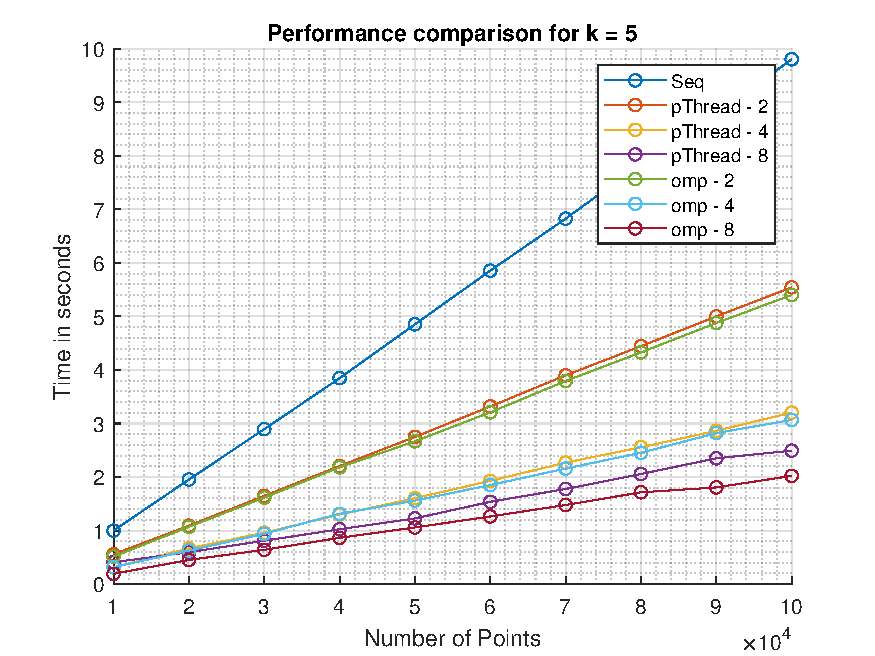
\includegraphics[width=7.8cm,height=6cm]{k5}
    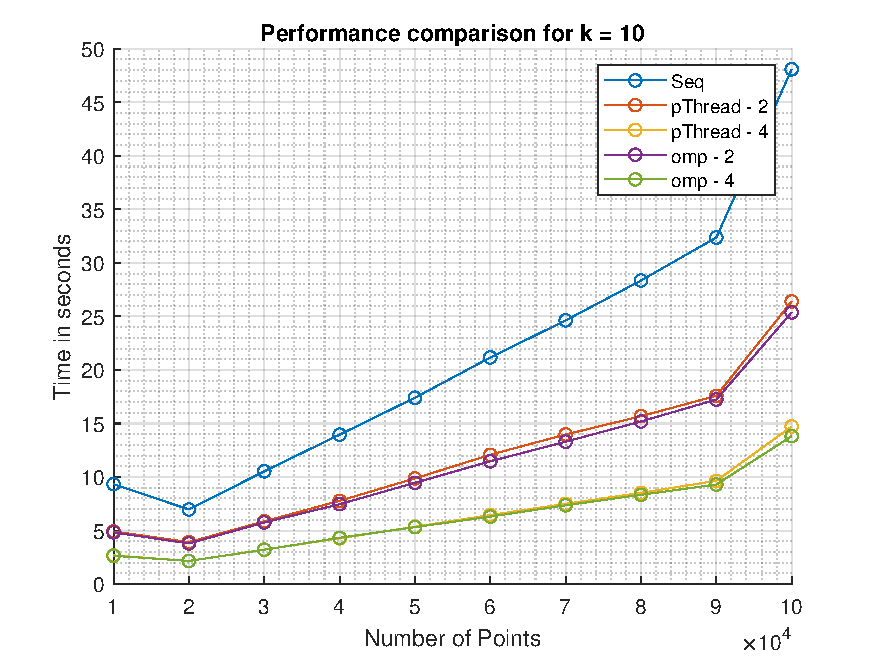
\includegraphics[width=7.8cm,height=6cm]{k10} \\
    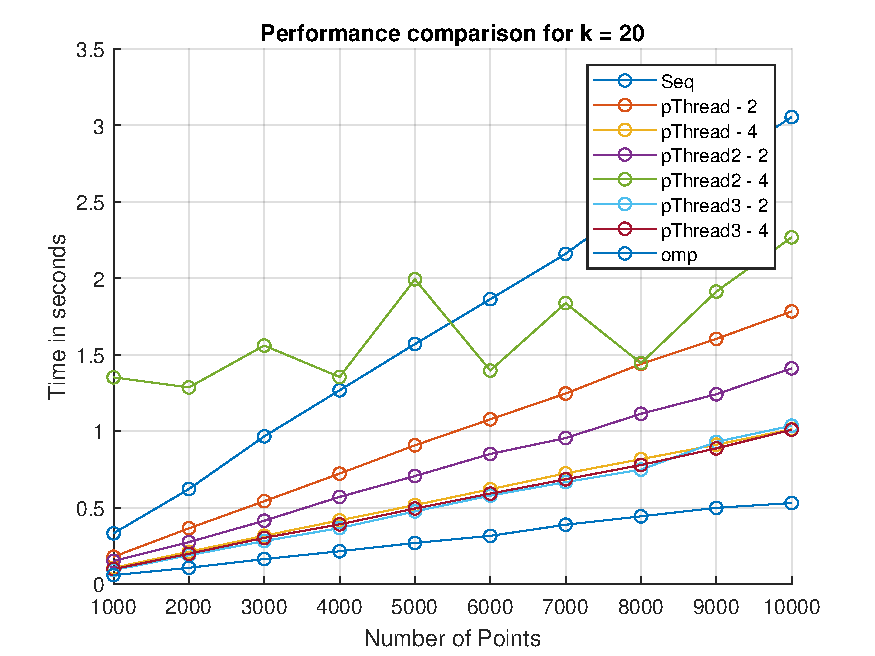
\includegraphics[width=7.8cm,height=6cm]{k20}
    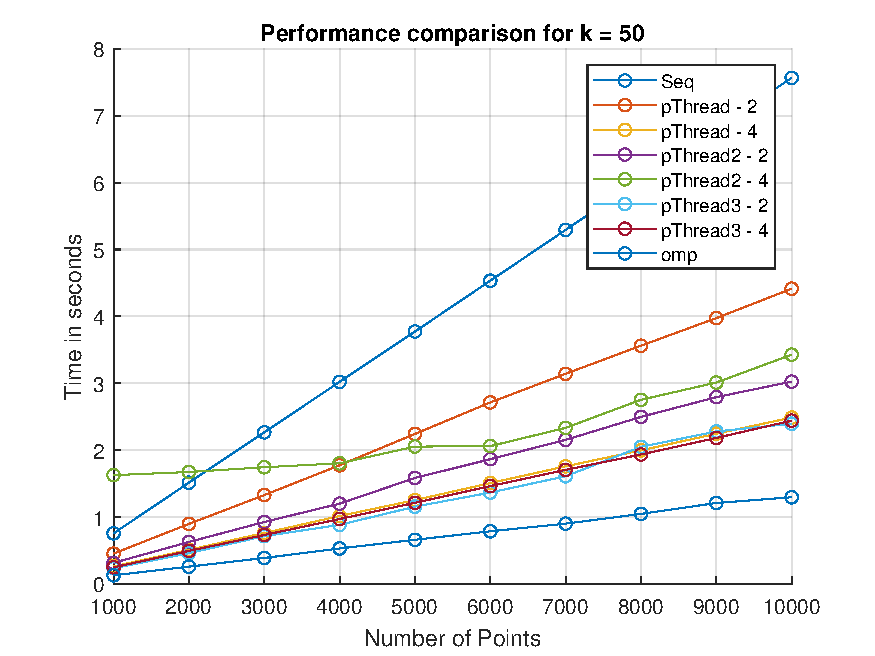
\includegraphics[width=7.8cm,height=6cm]{k50} \\
    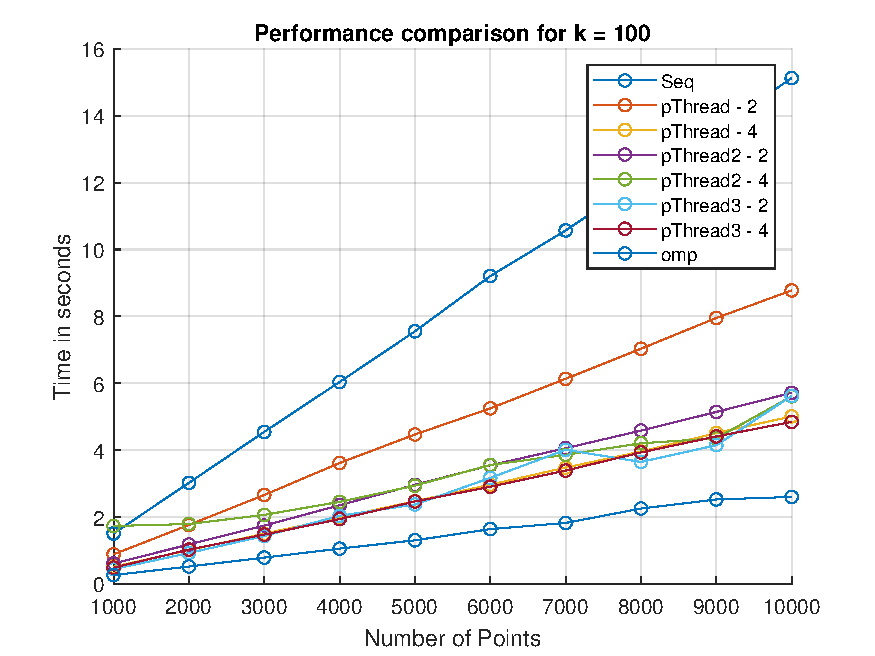
\includegraphics[width=8.5cm,height=6.5cm]{k100}
    \caption{Graphs showing time taken by different implementations for different k}
    \label{fig:my_label}
\end{figure}

\newpage
\section{Experiments}

To test the impact and efficiency of parallelisation in all the approaches we performed tests/experiments on the completion time of each implementation.

\subsection{Test setup}
The tests were run on the following setup:
\begin{itemize}
    \item Intel i7 7700K quad core processor hyper threaded to 8 virtual cores
    \item Cache line size = 64 Bytes
    \item Level 1 cache = 4 x 32 KB 8-way set associative instruction caches, 4 x 32 KB 8-way set associative data caches
    \item Level 2 cache = 4 x 256 KB 4-way set associative caches
    \item Level 3 cache = 8 MB 16-way set associative shared cache
\end{itemize}

\subsection{Observations and results}

The graphs in Figure \ref{fig:my_label} show the comparison between different parallelized implementations. We can conclude the following:

\begin{itemize}
    \item We first observe that all execution times grow linearly with problem size = number of data points.
    \item The execution time also increases as the number of cluster = K increases.
    \item We lso that the speedup in pThread case is around 1.9 for 2 threads (in light red) and around 3.7 for 4 threads (in yellow). 
    \item The pThread2 having high thread synchronisation overhead shows poor performance (in green) for small size K and nearly 2 speedup in 4 thread case.
    \item The OpenMP implementation gives nearly 6 speedup for the 4 thread run (in dark blue).
\end{itemize}






\end{document}
